\section{Our Method}
\label{sec:method}

\begin{figure}[b!]
\centering
\includegraphics[width=0.9\linewidth]{figures/bev_projection.jpg}
\caption{We visualize our BEV project process. Given a BEV semantic map $\textit{B}$, we project it to multiple perspective views. We overlay the semantics on the original RGB images in perspective view for better comparison.  
}
\label{fig:bev_proj}
\end{figure}

Our method aims to generate multi-view perspective images from text prompts given pixel-level BEV semantic correspondences. Specifically, we denote the BEV semantics as $\textit{B}\in\mathbb{R}^{H_b\times W_b\times c_b}$, with the ego car assumed to be located at the center. And $H_b$, $W_b$, and $c_b$ are the height, width, and number of semantic classes of $\textit{B}$, respectively. Our goal is to generate a set of perspective RGB images with resolution $H$ by $W$, or $\{I_m\}_m$ in particular, under $M$ virtual camera views. And the $m$-th perspective image is referred to as $I_m\in\mathbb{R}^{H\times W\times 3}$ where $m=\{1,\dots,M\}$. In particular, we assume the intrinsics, extrinsic rotation, and translation of the $m$-th camera are given and denote them as $K_m$, $R_m$, and $T_m$, respectively. 

As described above, we obtain visually coherent multi-view images by leveraging both global and local consistency in implicit and explicit manners. Specifically, our method consists of two stages. Our first stage takes BEV semantics $\textit{B}$ as well as $\{K_m,R_m,T_m\}_m$ as input and projects BEV semantics to each perspective view w.r.t. its camera parameter set, denoting as $S_m\in\mathbb{R}^{H\times W\times c_b}$ for the $m$-th view. The second stage parses $\{S_m\}_{m=1}^M$ and text prompts as input. And it produces RGB images from $M$ perspective views. $I_m$ denotes the generated RGB image from $m$-th view. 
% Thanks to the multi-view consistency module, our second stage is capable of implicitly leveraging global visual consistency among overlapping views when producing $M$ perspective RGB images according to perspective semantics and text prompts. 
%or $\{I_m\}_{m=1}^M.$ 
%Then the perspective semantics are stitched together according to the homography between overlapping camera views, leading to $\hat{S}_m\in\mathbb{R}^{\hat{H}\times\hat{W}\times c_b}$. 
More specifically, our first projection stage enforces global semantic consistency between BEV and perspective view explicitly with the help of geometric transformation. Meanwhile, the generation stage imposes consistency implicitly among overlapping perspective views with a multi-view attention module. Finally, we propose to explicitly enforce the visual cues at overlapping FOVs to be coherent with our novel training initialization and de-noising designs. The overall pipeline of MVPbev can be found in Fig.~\ref{fig:main}. We provide more details of the first and second stages in Sec.~\ref{sec:pers_map} and Sec.~\ref{sec:model} respectively. And the model training process is described in Sec.~\ref{sec:model_train}.

%The second stage of our method then parses the generated semantics $\hat{S}_m$ and text prompt, and produces multi-view images $\{I_m\}_m$. Specifically, we would highlight our homographic transformation module, which aims to enforce homographic constraints across multi-view feature maps. Details of the second step can be found in Sec.~\ref{sec:model}.

% We introduce the first step which aims to enforce cross-view consistency by generating corresponding semantics in Sec.~\ref{sec:pers_map}. Later on, our second step receives the generated semantics as well as paired text description, and produces multi-view consistent images. Details of the second step can be found in Sec.~\ref{sec:model}.

\subsection{Semantic-consistent view projection}\label{sec:pers_map}
Assuming that diverse yet plausible BEV semantics $\textit{B}$ can be obtained effortlessly with existing simulation methods~\cite{Wang_2019_CVPR}, the first fundamental problem that our method should address is to maintain cross-view semantic consistency from $\textit{B}$ to perspective images $\{I_m\}_m$. Secondly, contents at overlapping FOVs should also be coherent. For example, not only the background classes, such as buildings or trees, but also the foreground road participants, should be of similar appearance when they appear in different views. To this end, we first propose to project BEV semantics to $M$ perspectives view with camera parameters, which generates $\{S_m\}_{m=1}^M$ perspective semantics. Compared to existing work~\cite{zhang2023adding}, our projection step ensures semantic-wise consistency between BEV and perspective views with the help of geometry constraints, leading to fewer accumulative errors at the generation step (See examples in Fig.~\ref{fig:bev_proj}). % And our projection results can be found in Fig.~\ref{fig:bev_proj}.  

\subsection{View consistent image generation}\label{sec:model}
%Though being well-motivated and proved to be effective in terms of handling foreground objects~\cite{??}, 
Simply working on individual perspective semantics may lead to inconsistent content across different views, especially at overlapping FOVs. For instance, the buildings and the vegetation that appear at the FOVs among multiple views, e.g., the front, front-right, back, and back-left, have different appearances. This is due to the lack of interactions among cross-view cameras. We would like to note that such inconsistency would be reflected by neither BEV layout segmentation nor object detection metrics as it has influences on background classes only. 

Motivated by this, we propose to focus on these overlapping areas both methodologically and experimentally. As for our method, we apply strong coherency constraints on the background content by estimating the homography of overlapping areas, followed by a multi-view attention module to implicitly enforce the styles at various views to be coherent w.r.t. estimated corresponding points. 
% Moreover, we introduce novel initialization and de-noising processes to explicitly enforce latent features at overlapping areas to be consistent. 
%Later on, our generation stage works on the stitched images rather than the individual ones (See Sec.~\ref{sec:model} for more details). 
In this case, appearance consistency can be enforced not only on the background layout areas where the semantics are provided, but also on the other regions where control signals are missing. 
As for the evaluation purpose, we introduce human analysis to provide reliable evaluations on whether the generated images, especially the overlapping regions, are realistic or not. We demonstrate that our proposed method copes with background consistency well (See Sec.\ref{sec:experiment} for quantitative and qualitative results).

% \noindent{\textbf{Homography estimation}} 
\noindent{\textbf{Homography estimation}} We take the initial step towards enforcing visual consistency at overlapping FOVs by estimating the overlapping regions. To this end, we propose to compute the homography between images with overlapping FOVs. As illustrated in many driving datasets, one view generally overlaps with views on its left and right sides. Therefore, for the $m$-th view, we only need to consider $m_l=\mod(m+M-2,M)+1$ and $m_r=\mod(m+1,M)$, which are the left and right views of the $m$-th view respectively. Then we estimate the homography from view $m_r$ to view $m$ and denote the mapping function as $H_m$. Consequently, the $p=[x,y]$ coordinate in the $m$-th view will be mapped to coordinate $\hat{p}=[\hat{x},\hat{y}]$ in view $m_r$. Or $\hat{p}=H_m(p)$. Similarly, we define an inverse mapping $\overline{H}_m$ that maps $\hat{p}$ in $I_{m_r}$ to $p$ in $I_{m}$. 

%Denoting the left and right views of the $m$-th view as $m_l=\mod(m+M-2,M)+1$ and $m_r=\mod(m+1,M)$ respectively, 

% We provide one set of examples of our estimated homography in \textcolor{red}{Fig.~\ref{??}}. As can be found in this figure, our estimated homography is of high quality as we are able to generate reasonable results when stitching images with it. 

\begin{figure}[ht]
\centering
\includegraphics[width=0.9\linewidth]{figures/cross_view_attention.png}
\caption{Our multi-view attention module implicitly exploits the cross-view consistency by aggregating information from the target feature pixels in neighbour views.
% w.r.t. estimated homography. 
%Specifically, it aggregates information from the target feature pixels in neighbour views, which are obtained by homographic transformation, to the source.
}
\label{fig:cross_view}
\end{figure}

% \noindent{\textbf{Multi-view attention module}} 
\noindent{\textbf{Multi-view attention module}} What makes a set of views unrealistic? The first and foremost thing is the incoherence among images. In other words, realistic ones must appear consistent, as if they were taken in the same physical location at the same time of a day. More specifically, the visual styling of this set of images needs to be consistent such that all of them appear to be created in the same geographical area (e.g., urban vs. rural), time of day, with the same weather conditions, and so on. To this end, we introduce a multi-view attention module such that when generating the RGB from the $m$-th view, the views on its left and right sides 
% , or view $m_l=\mod(m+M-2,M)+1$ and view $m_r=\mod(m+1,M)$ respectively, 
% ~\footnote{Mathematically, the left and right views of the $m$-th frame should be $\mod(m+M-2,M)+1$ and $\mod(m+1,M)$. We }
are considered. For a token located at position $p$ in the feature
map $F_m$ generated from $m$-th view, we compute the attention output based on the corresponding pixels $K(\hat{p})$ in the feature maps generated by view $\bar{m}\in\{m_r,m_l\}$, where $\hat{p}^*\in K(\hat{p})$ denotes a $K$ by $K$ region centered at $\hat{p}$. Mathematically, we follow a similar formulation as in~\cite{vaswani2017attention} and define our multi-view attention module as:
\begin{equation} 
\mathbf{a}=\sum_{\bar{m}}\sum_{\hat{p}^*}Softmax(\left[Q F_m(p)\right]\cdot\left[K\bar{F}_{\bar{m}}(\hat{p}^*)\right]) V\bar{F}_{\bar{m}}(\hat{p}^*),~\label{equ:global_term}
\end{equation}
where $Q$, $K$, and $V$ are the learnable weights of query, key, and value matrices respectively. $\bar{F}_{\bar{m}}(\hat{p}^*)=F_{\bar{m}}(\hat{p}^*)+d(\overline{H}_m(\hat{p}^*)-p)$. We further denote $d(\cdot)$ as a position encoding to the $F_{\bar{m}}(\hat{p}^*)$ based on the 2D displacement between $p$ and $\overline{H}_m(\hat{p}^*)$. As can be found in Eq.~\ref{equ:global_term}, our multi-view attention module aims to aggregate information from the target feature pixels $K(\hat{p})$ to $p$. We provide a simple illustration of our multi-view attention module in Fig.~\ref{fig:cross_view}.

\subsection{Model training and inference}~\label{sec:model_train}
To train our model, we introduce a multi-view Latent Diffusion Models (LDMs)~\cite{rombach2021highresolution} loss. Basically, the original LDMs consist of a variational autoencoder (VAE) with encoder $\mathcal{E}$ and decoder $\mathcal{D}$, a denoising network $\delta_{\theta}$ and a condition encoder $\tau_{\theta}$. The input image $I_m$ is mapped to a latent space by $\mathbf{l}_m=\varepsilon(I_m)$, where $\mathbf{l}_m\in\mathbb{R}^{h\times w\times c}$. We follow the routine to set $\frac{H}{h}=\frac{W}{w}$ and they both equal to 8. Later on, the latents will be converted back to the image space by $\tilde{I}_m=\mathcal{D}(\mathbf{l}_m)$. The denoising network $\delta_{\theta}$ is a time-conditional UNet, which leverages cross-attention mechanisms to incorporate the condition encoding $\tau_{\theta}(\mathbf{c})$. In our case, $\mathbf{c}$ consists of text-prompt and semantics in perspective view $S_m$. 

\begin{figure}[t]
\centering
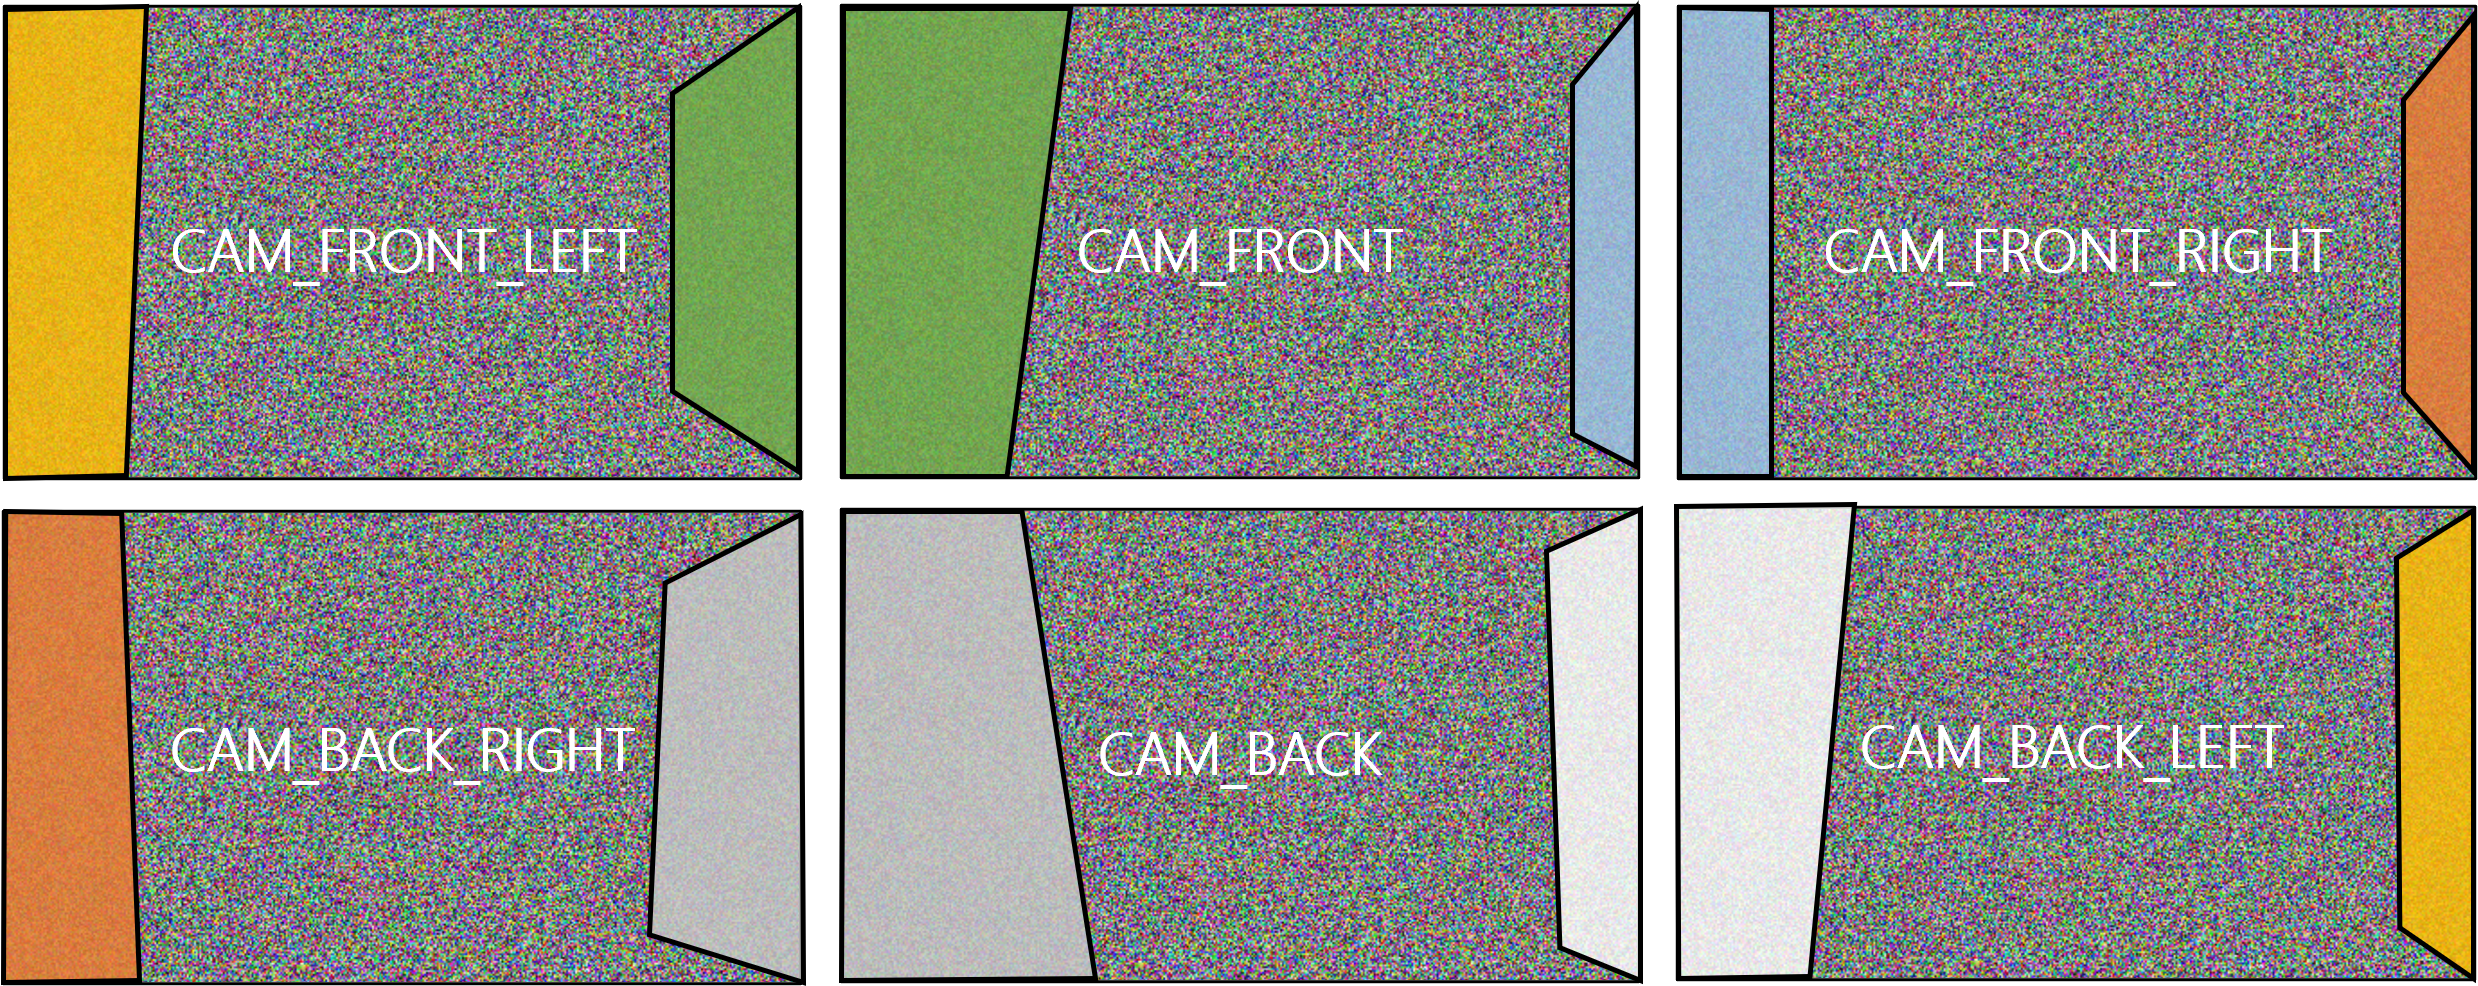
\includegraphics[width=0.9\linewidth]{figures/latent_initialization.png}
\caption{We explicitly enforce that the noise value of pixels at overlapping FOV should be consistent across views. 
}
\label{fig:noise_init}
\end{figure}

For each training step, we firstly uniformly sample a shared noise level $t$ from 1 to $T$ for all the multi-view images $\{I_m\}_{m=1}^M$, denoting them as $\{\epsilon^t_m\}_m$. And $\epsilon^t_m\sim\mathcal{N}(0,1)$. To leverage the cross-view consistency, we further enforce these noises to be the same if they correspond to the same pixel. Starting from the first view, or $m=1$, we re-assign value at coordinate $x,y$ of $\epsilon^t_m$, or $\epsilon^t_m(x,y)$, to $\epsilon^t_{m_r}(\hat{x},\hat{y})$. And we repeat the process until $m_r=1$. We provide one example set of our initialized $\{\epsilon^t_m\}_{m=1}^M$ in Fig.~\ref{fig:noise_init}. Finally, our model training objective is defined as:
\begin{equation}
\begin{aligned} 
 \mathcal{L}:=\mathbb{E}_{\{\mathbf{l}_m,\epsilon^t_m\}_{m=1}^M,t,\mathbf{c}}\left[\sum_{m=1}^M\|\epsilon^t_m-\delta_{\theta}^m(\{l_m^t\},t,\tau_{\theta}(\mathbf{c})\|_2^2\right],
 \end{aligned}~\label{equ:loss}
\end{equation}
where $\delta_{\theta}^m$ is the estimated noise for the $m$-th image. And we use $l_m^t$ to denote the noisy latent for the $m$-th image. 

At sampling time, the denoising (reverse) process generates samples in the latent space, and the decoder $\mathcal{D}$ produces RGB images with a single forward pass. To incorporate our idea that pixels at overlapping regions should be visually similar even at different views, we again employ the value assignment process. Similar to the noise initialization step, we re-assign value at coordinate $x,y$ of $l^t_m$, or $l^t_m(x,y)$, to $l^t_{m_r}(\hat{x},\hat{y})$. This re-assignment starts from $m=1$ and does not stop until $m_r$ equals to 1. In experiments, we observe that our design would improve the visual results if applied to up to $\frac{3\times T}{5}$ denoising steps. Otherwise, the performance deteriorates. % More steps would deteriorate the overall performance. 
% We provide some examples in Fig.~\ref{fig:denoise} as a reference. 

% \begin{figure}[ht]
% \centering
% \includegraphics[width=\linewidth]{figures/explicit_enforce_consistency.png}
% \caption{By explicitly enforcing the consistency in latents during denoising process, we are able to obtain more visually consistent results at overlapping areas. 
% }
% \label{fig:denoise}
% \end{figure}

% \begin{figure}[ht]
% \centering
% \includegraphics[width=\linewidth]{figures/obj_control_method.jpg}
% \caption{Our method to achieve test-time controlability by combining multiple attention responses from paired instance masks and text description, in a training-free manner.
% }
% \label{fig:control_method}
% \end{figure}

\noindent{\textbf{Inference}} As claimed in above, MVPbev can be extended with instance-level controllability. Specifically, Our MVPbev allows the user to click on the target instance and provide color-specific requirements. To achieve this, we propose a special mechanism for multiple foreground objects control, which manipulates the response of cross-attention layers to accurately guide instance-level synthesis. Assuming that instance-level masks can be obtained at each view with either existing methods~\cite{cheng2022masked} or simple retrieval. Specifically, we first obtain the instance-level and scene-level latents individually with its paired prompt. Then they are effectively combined with those binary instance-level mask, leading to more spatial-consistent performance. 
%as paired text description and instance masks are passed to cross-attention layers, multiple instance-level prompts and one scene-level prompt that we already have are individually feed to certain cross-attention modules. Later on, instance masks are incorporated to effectively combine the response from those cross-attention modules, with text description and objects location aligned. In this way, it becomes possible to control multiple objects separately. 
Please note that such ability on foreground objects of MVPbev are training-free, leading to far better extendability and test-time controllability. We refer the readers to supplementary for more details.

% Specifically, as paired text description and instance masks are passed to cross-attention layers, multiple instance-level prompts and one scene-level prompt that we already have are individually feed to certain cross-attention modules. Later on, instance masks are incorporated to effectively combine the response from those cross-attention modules, with text description and objects location aligned. In this way, it becomes possible to control multiple objects separately. Please note that such ability on foreground objects of MVPbev are training-free, leading to far better extendability and test-time controllability 
% (See Fig.~\ref{fig:control_method})}

% \noindent{\textbf{Inference}} As claimed in above, MVPbev can be extended with instance-level controllability. Specifically, Our MVPbev allows the user to click on the target instance and provide color-specific requirements. To achieve this, we propose to denoise the background stuffs and foreground objects individually at initial denoising steps, then instance masks are incorporated as attentions to effective combine latents from both, finally the combined latents are denoised together. Please note that such ability on foreground objects of MVPbev are training-free, leading to far better extendability and test-time controllability (See Fig.~\ref{??})